\section{Implementaci\'on existente}
\label{implementacion}

Antes de describir las mejoras realizadas sobre la aplicaci\'on existente, vamos a ver
los pasos que componen la construcci\'on de la matriz de Kohn-Sham, necesario para el
c\'alculo de la estructura electr\'onica.

\begin{figure}[htbp]
   \centering
   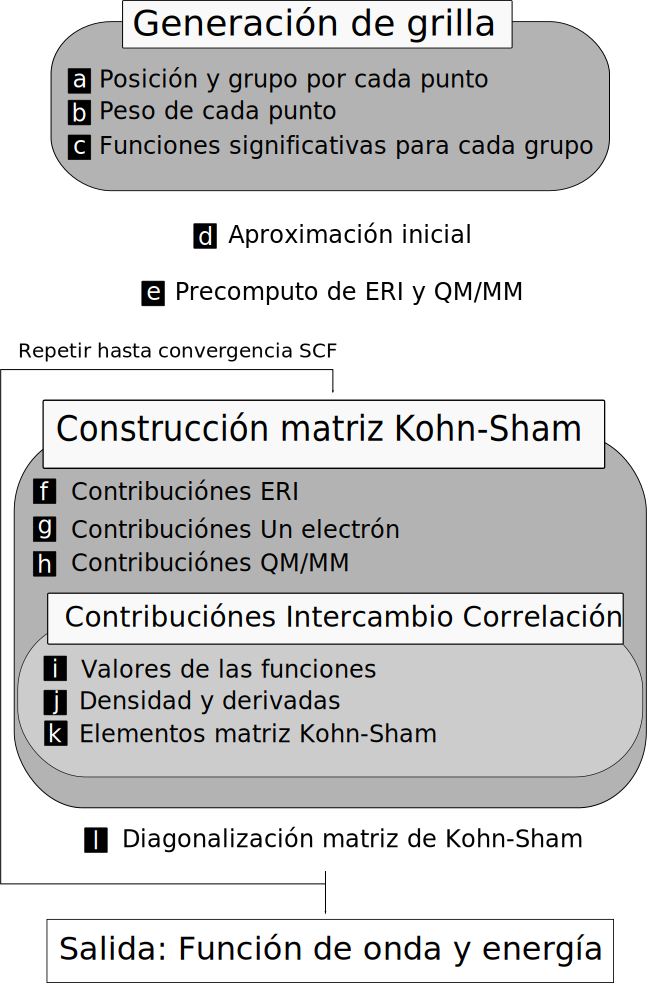
\includegraphics[width=250px]{images/g2g-steps.pdf}
   \caption{Pasos del c\'alculo de DFT realizado por LIO.}
   \label{fig:lio-steps}
\end{figure}

\begin{figure}[htbp]
   \centering
   \includegraphics[width=100px]{images/grilla.pdf}
   \caption{Esquema del mallado de integracion, partido en cubos y esferas para un sistema de dos \'atomos.}
   \label{fig:grilla}
\end{figure}
%En este trabajo nos vamos a concentrar en los puntos ijk que mas tardan
%Usamos la ecuacion \ref{approx_excenergy} aca
%Para calcular la densidad en cada punto, usamos la \rho^k que esta en cuda
%Hay que traerla aca para escribir la densidad, y explicar porque hacemos agrupamiento
%esto es porque las funciones son gaussianas y no son importantes en todo el espacio (si localmente)
% para cada punto entonces va a habar un grpo de funciones gaussianas que sean significativas,
% en vez de armar una lista para cada punto, si los agrupo espacialmente podes tener una lista que
% englobe a todos los puntos va a tener menor overhead que tener una lista para cada punto

Este esquema esta basado en el trabajo de Stratmann~\cite{Stratmann}, donde se propone
agrupar puntos de la grilla en vez de resolver el computo uno por uno. El agrupamiento permite determinar
cuales funciones tienen una contribuci\'on significativa al computo final. Dado que las
funciones Gaussianas decaen r\'apidamente a la distancia, el tama\~no del conjunto de
funciones significativas no depende del n\'umero de \'atomos del sistema. Es decir, el tama\~no
tiene orden constante en t\'erminos de complejidad computacional. Como consecuencia, es posible
subdividir el c\'alculo de la DFT computando los grupos de puntos de manera independientemente.

Para construir estos grupos se genera un mallado en cubos y esferas que incluya todos los puntos
de la grilla. Como los puntos no se distribuyen homog\'eneamente, sino que la mayor cantidad de ellos
se concentran cerca de los n\'ucleos, si se usara una partici\'on \'unicamente basada en cubos, la cantidad
de puntos contenidos en cada grupo diferir\'ia considerablemente. El uso de grupos esf\'ericos rodeando
los nucleos eliminan zonas de alta concentraci\'on de puntos y permite que los puntos remanentes
tengan una distribuci\'on mas homog\'enea. Este esquema de construcci\'on se muestra en la figura~\ref{fig:grilla}
y el detalle algor\'itmico de la generaci\'on se estudi\'o previamente~\cite{Nitsche2014,TesisNitsche},
sin modificaciones para este trabajo.

Un diagrama simplificando la estructura del c\'alculo de DFT se puede ver en la figura \ref{fig:lio-steps}.
Los pasos (a) a (e) corresponden a la etapa de inicializaci\'on, y se calculan una \'unica vez
al comienzo de la simulaci\'on. La iteraci\'on de SCF (\textit{Self-Consistent Field}) se
compone de los pasos (f) a (l). Este ciclo se repite mientras la matriz densidad cambia
m\'as de una cierta tolerancia previamente establecida.~\cite{Nitsche2014}.

Los pasos de la figura \ref{fig:lio-steps} m\'as computacionalmente costosos son (i), (j) y (k).
En la implementaci\'on original de LIO~\cite{TesisNitsche}, se muestra como estos pasos
obtienen grandes mejoras en GPU sobre su implementaci\'on de referencia en CPU. Sin embargo,
estos pasos todav\'ia insumen una gran cantidad de tiempo, incluso en las versiones aceleradas.

A continuaci\'on se presentan distintos cambios hechos a las rutinas para minimizar los tiempos,
sin cambiar la estructura general del c\'alculo, ya probado en la literatura.

\section{Implementaci\'on en CUDA}

\subsection{Estructura inicial del programa}

El programa originalmente estaba concebido para ser corrido en GPU nVidia GTX8800.
Luego, las cosas que se usaron para este desarrollo consistieron en la libreria CUDA version
2, para arquitecturas a lo sumo SM20.

La estructura del programa era la siguiente:
\begin{enumerate}
\item Se determinan los mallados del sistema
\item Se clasifican en cubos y esferas
\item Para cada elemento, se resuelve el sistema
\item Esto se repite hasta que converga a lo sumo en una cantidad limitada de pasos, o diverga
\end{enumerate}

La resoluci\'on del sistema en si esta compuesta de varios pasos:
\begin{enumerate}
\item Se obtiene el valor de la funci\'on de onda en cada punto de la malla
\item Se generan las matrices con los gradientes y los hessianos de cada funci\'on
\item Se calculan las densidades y el producto matricial por bloques por funci\'on
\item Se calcula la matriz de coeficientes de las fuerzas entre las particulas
\end{enumerate}


\subsection{Cuellos de botellas originales, limitantes estructurales}

El cuello de botella principal que presentaba este c\'odigo era en la
resoluci\'on del sistema, especificamente en el c\'odigo que calculaba la matriz de Kohn-Sham.
En el GPU, esta funci\'on insumia el 95\% del tiempo total, que en sistemas de gran cantidad
de puntos, estaba en el orden de minutos. Los problemas principales que mostraba esta funci\'on fueron:
\begin{itemize}
\item Cantidad de accesos a memoria global
\item Falta de accesos coalescentes
\item Sobreuso de la memoria compartida
\item Subsaturacion de los SM
\end{itemize}

\subsection{Accesos a memoria global}

\subsection{Falta de accesos coalescentes}
Asi como a los CPU les interesa realizar accesos alineados a memoria, a los GPU les
interesa aun mas. El termino coalescencia de memoria se aplica a GPU mediante
la organizacion de los accesos a memoria de manera ordenada y predecible. La l\'ogica
detras de esto es que cuando el GPU accede a memoria de manera alineada, puede traer
entre 16 y 64 bytes en una sola lectura, mientras que si debe acceder de manera no
alineada a memoria, o con threads que no acceden de manera predecible a esta, entonces
se deberan serializar los accesos y separar en m\'ultiples accesos a memoria global para leer
esta informaci\'on. Este problema solamente se agrava si se debe hacer muy frecuentemente
por cientos de threads, como es el caso de los bloques con gran nivel de paralelismo explicito.

\subsection{Sobreuso de la memoria compartida}

Los SM cuentan con una memoria compartida entre todos los threads, la memoria shared. Esta
tiene un bus de baja latencia con conexionado especifico dentro de cada SM.

\subsection{Subsaturacion de los SM}
La subsaturacion de los SM se da en los casos donde haya SM que esten listos para correr
c\'odigo pero que no puedan hacerlo porque tienen contencion en algunos de sus recursos.
La m\'etrica usada para determinar esta saturaci\'on es la ocupancia de los SP.
Esta es la proporci\'on de threads activos sobre el total de threads disponibles de un bloque.

Existen en esta arquitectura principalmentre tres recursos que, en un principio, parecen
ilimitados pero en realidad son finitos y compartidos por los procesadores de la GPGPU.
Estos son:
\begin{itemize}
\item Cantidad total de threads por bloque.
\item Cantidad total de registros usados por thread.
\item Cantidad de memoria compartida por bloque.
\end{itemize}

El mecanismo de scheduling de los SM funciona asignando un bloque a cada SM, que
va a correr sin preemption hasta que terminen todos sus threads asignados. Idealmente, cada
bloque cuenta con una cantidad de threads suficiente para poder esconder la latencia
de las ejecuciones mediante un cambio de contexto. La arquitectura GPGPU esta dise\~nada
para este fin, por lo cual se cuenta con un mecanismo de cambio de contexto de costo cero~\cite{NvidiaFermi} para
poder empezar a correr los threads de un warp diferente, del mismo bloque.
Si el bloque no cuenta con suficiente cantidad de threads para poner a correr de manera
concurrente, el SM va a forzosamente esperar que finalicen las operaciones de alta latencia
de estos warps sin nada que hacer mientras tanto. Si, por el contrario, se contasen con
miles de threads por bloque, entonces es posible que las operaciones que sirvan
para sincronizar los threads de todo un bloque en un punto espec\'ifico antes de proseguir
(un barrier) sean excesivamente costosas.

La arquitectura GPGPU de NVIDIA organiza los registros de todos los threads en un unico
register file, com\'un a todos los bloques. Como cada thread usa decenas de registros para guardar
los computos intermedios, NVIDIA decidio unificarlos, ya que es muy variable la cantidad que va a usar
cada kernel de ejecuci\'on. Una de las grandes diferencias entre Fermi y Kepler es la cantidad m\'axima de
registros por thread. Mientras que Fermi permitia hasta 63 registros, Kepler permite hasta 255. Esto
es positivo para poder correr bloques de pocos threads pero gran cantidad de registros. Por otro lado,
aumenta la presion sobre el register file. Cuando se lanzan muchos threads
que puedan estar corriendo paralelamente entre todos los SM de la GPU, es posible que se supere
la cantidad m\'axima de registros presentes en el register file. Esto fuerza a que el scheduler
no pueda poner a ejecutar m\'as bloques que los que pueda soportar este recurso, dejando SP ociosos.

Finalmente, al igual que con los registros, la memoria compartida es un recurso limitado. Como
solamente se cuenta con hasta 48Kb (Fermi-Kepler) de memoria de este tipo para ser repartida entre
todos los bloques que esten corriendo en todos los SM, el scheduler debera decidir no poner a ejecutar
m\'as bloques simultanemante que los que pueda soportar la cantidad de memoria compartida.

El problema tratado dentro de esta tesis cont\'o con todos estos limitantes. Afortunadamente,
las herramientas de profiling usadas remarca estos limitantes constamente, haciendolas
fundamentales a la hora de evaluar como proseguir en la busqueda de optimizaciones de c\'odigo.

\subsection{Cambios en el threading}
%Cambiamos de blocks por puntos, a blocks por funci\'on.
De los 3 kernels que originalmente componian la iteracion de SCF, el que se encargaba
del calculo de la densidad insumia el 94\% del tiempo total de uso de la GPU. Minimizar
el tiempo de ejecuci\'on de esta funcion resultaba vital para poder disminuir el tiempo
de convergencia de SCF.

El cuello de botella fundamental radicaba en como se distribuia el trabajo de computo
entre los kernels. La estrategia de paralelizaci\'on original determinaba la partici\'on
del sistema a resolver instanciando un bloque por cada punto (\texttt{blockId.x $\in$ group\_m}),
una cantidad fija de threads (usando \texttt{threadId.x $\in$ BLOCK\_SIZE})
Los threads servian para reutilizar la memoria compartida; cada uno hacia la lectura
de un $F_i$ que se lo compartian entre todos, y luego todos usaban un $F_j$ distinto, para
hacer la multiplicaci\'on de filas por columnas.

Esta distribuci\'on resultaba natural al problema, pero visto con mayor detalle, esto
implicaba una cantidad de cuentas innecesarias que podian ser eliminadas.

Uno de los cambios importantes fue crear mas bloques, para las particiones que tienen
mas funciones. Decidimos usar otra dimensi\'on de los bloques (\texttt{blockId.y}),
para determinar cuantos grupos de threads van a hacer falta para procesar completamente
todas las funciones de ese punto. Llamamos a este parametro $altura\_bloques$. Se
calcula para cada particion entonces como $altura\_bloques = {group\_m}/{BLOCK\_SIZE}$
Para todas las particiones chicas, este valor no supera a 1. En los cubos y esferas m\'as
grandes (de los sistemas probados), la altura puede ser hasta 6. Esto significa una gran
cantidad de bloques adicionales con respecto al m\'etodo anterior.
%%
%%

Despues de haber hecho el cambio de la parelelizacion, estudiamos realizar
mas de un punto por thread. Esto sirve para aprovechar un par de lecturas que son comunes
entre dos funciones. Con este cambio, se instancian menos bloques (la mitad de la dimension $y$
definida para esto) y se pueden ocultar algunas latencias de acceso, pero
cada grupo de threads lleva m\'as tiempo y usan m\'as registros. Esta estrategia es similar
a un loop unrolling manual, aplicado a la arquitectura GPU.

Un punto de intensa discusion durante estos cambios es el valor de \textit{BLOCK\_SIZE}.
Para nuestro problema, decidimos utilizar un numero de threads por bloque m\'ultiplo del
tama\~no de un warp (32 threads). Esto permite estudiar como afectan en el tiempo de
procesamiento contar con uno o m\'as warps por bloque. Una ventaja de usar bloques de
32 threads, es que el costo de la sincronizaci\'on es exactamente cero. No se precisa
sincronizar nada puesto que los threads trabajan en lock-step sincronizados por warp.
Un bloque chico ademas nos permite usar mas memoria compartida por thread, dado que hay una
cantidad fija de memoria por bloque (entre 32Kb y 64Kb). Cuando se cuentan con muchos m\'as
threads, se debe reducir este uso por thread de modo que todos puedan ejecutar concurrentemente.

Dicho esto, la literatura ~\cite{farberCuda} sugiere siempre que sea posible
usar bloques grandes y con threads lo m\'as independientes posibles. Una gran cantidad de threads
en un bloque permite tener muchos m\'as warps para schedulear de modo de esconder las latencias de
operaciones y de a accesos globales. Sin embargo, contar con muchos threads hace que las
sincronizaciones sean mucho m\'as costosas. Ademas, como cada SM no cuenta con preemption
de bloques, contar con muchos threads por bloque hace que los recursos se mantengan
por largos periodos.

Inicialmente, este tama\~no se habia fijado en 128 threads por bloque, 4 warps. Utilizando
mas memoria compartida en el esquema de paralelizaci\'on para disminuir accesos a memoria global,
este valor resulto demasiado elevado y disminuia la posibilidad de ocupar todos los SM en dispositivos
Fermi y Kepler. Con solamente 32 threads, se podia maximizar la ocupacion de los SM, pero habia
muchos m\'as bloques. Finalmente, luego de disminuir un poco el uso de memoria compartida por
bloque, usando algunas ideas descriptas a continuaacion, pudimos fijar este valor en 64 threads
por bloque. Mostramos que tener solo un warp es bueno, pero mucho mejor a\'un es tener dos warps, porque
esto permite, con costo cero, poner a correr el otro para ocultar la latencia sin agrandar
demasiado el costo de la sincronizaci\'on.


%%%%%%%%%%%%% fruta underneath
Una cosa que se nota que este mecanismo de paralelizacion cuenta con
la ventaja de que casi no se compartian los datos entre los distintos threads, lo cual,
a priori, deberia haber ocasionado que no hubiera mucho mejor forma de realizar el computo.

Originalmente el c\'odigo generaba un bloque por cada punto en el grupo de puntos
que teniamos que solucionar, con una sola dimension por thread.
Como este era el kernel que insumia el 94\% del tiempo de todo el proceso, decidimos
atacarlo de raiz, cambiando la paralelizaci\'on. A pesar de que el profiler de CUDA nos indicaba
que tenia una buena occupancy, decidimos cambiar de fondo el encare del problema.


Sin embargo, con un detalle m\'as fino, es posible notar que este mecanismo hacia que
muchos threads hicieran cuentas innecesarias, que no contribuian a la reducci\'on total.
Esto daba una alta ocupancia ficticia, que buscamos acercar a la real. Adem\'as, a pesar
de que se compartian muy poca informaci\'on por la memoria compartida, tambien habia muchos
puntos de sincronización a nivel bloque.




\subsection{Cambios en la reducci\'on}
%Hubo que agregar reducci\'on de suma a nivel punto porque ya no se comparten mas la info
La reorganizacion de la paralelizacion del kernel del calculo de la densidad creo la necesidad
de varios pasos de reducci\'on que antes se hacian solos.

El primer paso, al ya no haber un bloque por punto, habra que totalizar el c\'alculo de la
suma de todos los elementos de la columna que acabamos de procesar para obtenerlo. Para reducir,
vamos a reutilizar la memoria shared que empleamos en el c\'alculo de la energia anterior. Cada
thread va a poner el valor final del computo realizado en su posicion correspondiente en el
la memoria compartida. Esto luego se ejecuta como una reducci\'on en \'arbol, donde cada
thread suma el valor de la posici\'on $x$ con el valor en $2*x$, si fuera este valido. Esto
luego se repite por la mitad de los threads, hasta que solo el thread 0 lo ejecuta,
generando exactamente un valor por bloque, que lo va a terminar escribiendo en la memoria
global.

Esta t\'ecnica de reducci\'on es sumamente conocida para arquitecturas distribuidas, generando
la respuesta en $O(log_2(n))$ pasos. La literatura de CUDA~\cite{cudaReductions} sugiere tecnicas adicionales para
minimizar a\'un mas el tiempo empleado en esta reducci\'on, pero considerando que hay, a lo sumo
6 operaciones, no hay necesidad de mejorar esto mas.

Como va a haber $altura\_{bloque}$ cantidad de escrituras para cada punto, va a entonces
hacer falta guardar estas cuentas parciales en memoria global. Para eso definimos una matriz
por cada uno de los parametros que debemos acumular, con tama\~no identico a la cantidad de bloques
del kernel \texttt{compute\_energy}, para que cada uno de estos escriba unicamente en una posici\'on
univocamente identificada de este. Estas matrices luego son de tama\~no $O(\#_{puntos} * altura_{bloque})$,
menos de 1Mb en el caso m\'as grande.

El siguiente paso de la reducci\'on consiste en acumular los $altura\_{bloque}$ valores descriptos
recien en un solo por punto. Esto implica encontrar donde estan en las matrices temporales las
partes de las cuentas, agregarlas y calcular el potencial correcto. Esto genera finalmente los
coeficientes para calcular la actualizaci\'on de la matriz de Kohn-Sham y los factores para el
c\'alculo de la matriz de fuerzas.

Esto se refleja en el c\'odigo como una llamada a un nuevo kernel adicional, posterior a la
cuenta de la densidad y con m\'ultiples matrices temporales adicionales. Este kernel es sumamente
eficiente porque ya todo el trabajo pesado lo hizo el anterior. Solo se tiene que realizar
a lo sumo $altura\_{bloque}$ sumas y una llamada a la funci\'on que calcula el potencial y densidad,
un kernel corto de alta intensidad aritm\'etica que realiza solamente operaciones matem\'aticas.
Finalmente, la acumulaci\'on finaliza, generando un valor por cada punto, lo mismo que se producia
anteriormente pero utilizando mucho mejor los recursos del dispositivo.

\subsection{Cambios en los accesos globales}
La arquitectura de las placas de video estan pensadas entorno al poder de computo.
Las decisiones tomadas por los diseñadores de las GPGPU se concentran alrededor
de paralelismo a lo ancho, poniendo un gran enfasis en la cantidad de nucleos. Luego,
se dispone de menor cantidad de espacio disponible en el die para las memorias.

Esta decision implica que la amplia mayoria de la memoria de la GPGPU se encuentra
localizada externa al procesador.  No solo esta fisicamente mas lejos, sino que
adem\'as la latencia para accederla es altisima. Es decir, el paradigma de
programaci\'on de las GPGPU gira entorno a esconder la gran latencia de los accesos
a las memorias globales.

Una de las memorias intermedias entre entre el procesador y la memoria global es
la memoria de textura. La memoria de textura es un cach\'e sobre la memoria global,
que esta focalizado alrededor de los accesos a memoria en varias dimensiones.
Estas memorias reciben su nombre de su funci\'on principal, que es en el area de los
sistemas de video. Los mapas de textura suelen ser grandes matrices que definen
tanto los colores sobre las superficies de los poligonos como los relieves.
El detalle crucial de estas memorias es que un miss en estas cache, provoca
que se traigan datos no solo contiguos en memoria, como pasa en las caches de
CPU normalmente, sino que ademas se traigan los datos en posiciones logicas contiguas,
es decir, variando las distintas dimensiones de la matriz subyacente.

Las memorias de textura se ajustan bien a los problemas de GPGPU, porque se relacionan
intimamente con los los mecanismos de paralelismo de CUDA. Como los problemas se pueden
dividir en bloques con threads en $x$, $y$, $z$, entonces tiene mucho sentido pensar
que las estructuras de datos subyacentes se van a acceder usando indices multidimensionales.

En nuestro problema, la memoria de textura se presenta como una soluci\'on para
los accesos bidimensionales de la matriz de RMM para el grupo de puntos.
Como esta matriz debe ser multiplicada por todos los valores de las funci\'ones,
derivadas primeras y segundas, se va a acceder a toda la matriz de RMM mas de
una vez por cada thread. Adem\'as, como se va a usar toda la matriz, y esta suele
tener un tamaño intermedio (es muy grande para memoria constante), el problema
suele entrar casi completamente en la memoria de textura.
La lectura bidimensional en este caso, se ajusta muy bien a los accesos por filas
y por columnas a la matriz.

El uso de la memoria de texturas agrega un recurso mas que tenemos que tener en
cuenta a la hora de profilear el c\'odigo. Para administrar los accesos a
la memoria de textura, cada multiprocesador tiene multiples "Unidades de textura".
Cuando dependemos de sobremanera de la memoria de textura para esconder la latencia,
se presentan contenciones sobre el acceso a las unidades de textura. Esto es
uno de los motivos por los cuales el procesador stallea los bloques hasta poder
ejecutarlos, cuando se liberan un poco mas los recursos.

%http://www.realworldtech.com/gt200/10/   << detalles sobre texture cache invalidation

\subsection{Cambios en los pasajes de informaci\'on intrawarp}
%Los shuffles que no anduvieron salvo en function
La arquitectura SM35, junto con CUDA5, trajeron aparejadas una herramienta interesante
para el manejo interno de los pasajes de informaci\'on intra-warp durante la ejecuci\'on.
Las instrucciones de shuffle, como asi las denomina NVIDIA, son instrucciones que facilitan
el pasaje directo de un registro de un thread en un warp, a otro, en un solo ciclo de ejecuci\'on.
Estas instrucciones existen en diversas maneras, con distintos propositos. Principalmente se
utilizan para pasar de un thread al siguiente (modulo el warp size) un registro para poder seguir
operando. Otro uso que puede tener mucho interes proximamente son las instrucciones de votaci\'on,
donde se evalua un predicado para todos los threads, y se setea o limpia un bit en el resultado
de respuesta si se cumplio el predicado para ese thread. Con esta herramienta, no es necesario
acceder a memoria compartida para poder pasar minima informaci\'on dentro de cada warp.

Nuestro uso de las funci\'ones de shuffle consistio en intentar eliminar lo m\'as que podiamos
los accesos a la memoria compartida, una fuente de bloqueos porque, a pesar de que ya corre
todos los bloques concurrentemente, leer elementos de ahi toman 4 ciclos en vez de uno solo
como en las funci\'ones de shuffle.

Probamos pasar de a un elemento y de a uno o dos vectores de 3 elementos, para comparar
cuan notable era el impacto del acceso mas veloz.

Finalmente concluimos que era una opcion valida para el pasaje de los valores de la funci\'on,
pero que el overhead de uso para cosas como los hessianos de la funci\'on no justifica el uso.
Adem\'as, como estas funci\'ones de shuffle solo estan presentes en las ultimas placas Kepler,
consideramos que el aprovechamiento marginal de los recursos no era lo suficientemente meritorio
de romper compatibilidad con las placas de la generacion Fermi anterior.


\subsection{Cambios en el almacenamiento de matrices temporales}
Una de las principales limitaciones de las GPGPU es la cantidad fija de memoria. Esta no es
expandible dado que esta soldada a la placa. Esto era aun m\'as notable cuando las placas
contaban con menos de 1Gb de memoria (A\~nos 2007-2008).
Para problemas de calculo num\'erico, esto era un limitante muy serio; los problemas que
normalmente entraban en la memoria principal de un CPU, no entraban completos en las GPU.
La decisi\'on tomada por muchas aplicaciones de entonces es compensar esto calculando
datos intermedios y tirandolos al final; teniendo que ser recalculados en las proximas iteraciones.

Esta estrategia es claramente impractica en CPU, puesto que se cuenta con mucha mas memoria
de uso general. En GPU era necesario por el faltante de memoria, pero no es tan notorio como en CPU,
puesto que estas cuentas se pueden hacer bastante m\'as rapido en GPU.

Cuando la aplicacion original se concibio, no habia siquiera placas Tesla de GPGPU apuntadas a HPC, con
m\'as memoria disponible que los modelos de consumidores. Aprovechando estos recursos actuales,
desarrollamos un m\'etodos para poder almacenar estos resultados temporales, de manera dinamica
durante la ejecuci\'on de la aplicaci\'on, para poder aprovechar este recurso que originalmente
era limitante pero ya no.

Para poder determinar que cosas van a ser guardadas en mem\'oria y que no, se determin\'o una heuristica
que define el orden de las particiones a solucionar. Esta heuristica estima que tama\~no van a
tener las matrices temporales a almacenar y ordena las particiones de menor a mayor. Esto
esta basado en el criterio de que, si bien es proporcional el tiempo de computo de estas matrices
temporales a la cantidad de funciones por grupo y cantidad de puntos (lo que determina el tama\~no
de la partici\'on), la constante es elevada. Determinamos entonces que es m\'as conveniente
aprovechar la memoria de la placa que almacena muchas matrices temporales de particiones chicas
a que almacene solamente un par de las grandes.

Para controlar la administracion de memoria, se realiza la estimaci\'on si la placa cuenta
con la suficiente memoria libre para guardar los datos a calcular, y si puede, se guardan de manera
permanente (hasta que la partici\'on se mueva a otro dispositivo o la liberaci\'on de recursos al
finalizar el programa). Esto ademas es configurable de modo que una corrida pueda usar un porcentaje
de la memoria con la que cuenta la placa, para poder correr multiples procesos de simulaci\'on concurrentemente.

Esta sencilla mejora permite explotar el hecho de que las placas hayan aumentado dramaticamente su
capacidad de almacenamiento, un recurso que hasta recientemente venia siendo un limitante podemos
convertirlo en una aceleraci\'on notoria.


\subsection{Cambios en las memorias compartidas}
%Cambiar los vec\_type4 por 3 en los accesos a la shared es mucho mejor, no hace falta alinear ahi
Otro de los problemas existentes del c\'odigo que quisimos atacar fue el mejor empleo de las
memorias shared. Estas son un recurso finito y muy importante, ya que son un limitante de
la ocupancia de los multiprocesadores. Como pueden correr una cantidad de bloques que, a lo sumo,
no superen los 48Kb de memoria shared simultaneamente entre todos, es imprescindible minimizar el
alocaci\'on de la memoria shared de modo que no estemos subutilizando los SM.

Una cosa que probamos, con un grado de exito variante, fue disminuir el tamaño de los vectores
donde almacenamos las derivadas direccionales. Como nuestro problema es en tres dimensiones,
y los vectores estaban configurados para tener 4 valores por cada derivada, probamos llevarlos a
3, para que se ajusten a su consumo real de memoria. Este acercamiento no consider\'o el porque
se hizo asi de esta manera originalmente. Tener 4 valores consecutivos en memoria fuerza
al compilador a alinearlos a 16/32 bytes (simple y doble precision).
Esto presenta grandes ventajas a la hora de hacer transferencias de memoria global en los accesos,
por lo cual decidimos dejarlo como estaban.

Sin embargo, este mismo criterio no aplica a las memorias shared de la GPGPU. Como los accesos
a estas memorias se realizan de a 4 bytes y no de a 16/32, entonces no tiene ninguna ventaja
en particular realizar el alineamiento; ya estan alineadas porque los elementos de cada punto
son flotantes de precisi\'on simple o doble (4 y 8 bytes respectivamente). Adicionalmente, como el
cuarto valor no tiene forma de marcarse como algo que no sea padding de alineaci\'on, todavia se
opera normalmente con el, por lo que eliminarlo ahorra una operaci\'on de c\'alculo. Mas a\'un,
se presentan una disminuci\'on del 25\% de los recursos de la memoria compartida por thread,
sin ninguna desventaja a la hora de acceder a estos. Principalmente esta mejora permite
aumentar la cantidad de bloques corriendo concurrentemente en los SM, al punto de eliminar
la limitaci\'on presente debido a las memorias compartidas.

\subsection{Cambios en los condicionales}
La arquitectura CUDA representa un m\'odelo de computo pensado en el procesamiento secuencial masivo
de datos de punto flotante. Esto es herencia de su legado de placa gr\'aficas, que era un stream
constante de datos. Al generalizar la arquitectura para que sea de proposito general, entonces
surge el problema de ejecuci\'on condicional. Como el resultado de la evaluaci\'on puede ser distinto
para cada thread, entonces surge el problema de como ejecutar un warp en lockstep cuando algunos threads
correran la rama \texttt{true} y otros la rama \texttt{false}. La soluci\'on que adopta CUDA es la
serializaci\'on implicita. Los threads que no ejecutan el \texttt{true} correr\'an \texttt{NOP}
y lo mismo se hara en el caso del \texttt{false}, al reves.

Esto trae aparejado una penalidad importante. Si esa bifurcacion contiene mucho c\'odigo no trivial,
entonces es evidente que se subutilizan importantemente los recursos disponibles.

Habiendo varios de estos casos en los kernels presentes, decidimos utilizar una t\'ecnica sugerida
por NVIDIA. Esta consiste en hacer las operaciones normalmente, como si todos los threads cumplieran
las condiciones del condicional y multiplicar por 1 o por 0 el resultado antes de acumular.
Esto hace que las cuentas que no se ejecutaban antes ahora lo hagan pero que simplemente no aporten
a la reducci\'on. Esta t\'ecnica elimina la existencia de la rama falsa de los condicionales, pero
trae dos problemas no triviales.

Uno de ellos es como solucionar el problema de los accesos a memoria.
Usualmente las guardas condicionales estan puestas para que el programa, si cumple ciertas condiciones,
no acceda a memoria que no esta definida. Por ejemplo, si \texttt{threadId > arraySize}, entonces claramente
no deberia acceder a \texttt{array[threadId]}, puesto que seria memoria invalida. Si eliminamos la guarda
entonces los accesos a memoria no pueden quedar igual. Una soluci\'on consiste en multiplicar tambien
por 1 o por 0 la direccion a la cual se va a acceder. Como CUDA maneja los arreglos de memoria
como C (es decir, basados en 0 como primer direcci\'on), esta t\'ecnica es v\'alida para hacer
siempre accesos correcto a memoria. El problema luego es en la coalescencia; como ahora algunos
threads de un warp van a acceder a una posicion de memoria muy distinta a otros, entonces el procesado
va a partir esos accesos en m\'ultiples transacciones. Esto puede hacer que la cuenta no solo no mejore
la performance, sino que puede que la empeore sustancialmente. Se debe hacer un profiling caso
por caso para poder estudiar el impacto en el kernel.

El otro problema es en cuentas que pueden dar NaN (como el tipico caso de division por cero).
Como, por estandar IEEE 754, los NaN hacen que todas las operaciones con ellos den NaN,
entonces pueden propagarse por la cuenta, incluso en con multiplicaci\'on con cero del resultado.
La soluci\'on m\'as evidante seria comprobar si son NaN antes de reducirlas, y si lo fueran, reemplazarlos
por cero. Esto puede llegar a ser inevitable en muchos casos, pero en el nuestro, si replanteamos
las cuentas, podemos evitar esos casos.

\subsection{Escalando m\'as all\'a de un GPU}
Una vez que fueron solucionados muchos limitantes de performance en los kernels del computo
de la densidad electr\'onica y del c\'alculo de la matriz RMM, nos encontramos en un punto donde
no fue posible determinar mejoras significativas en el c\'alculo para reducir tiempos.
Decidimos subir un nivel m\'as el paralelismo, de modo de poder solucionar multiples particiones
simultaneamente. Dado que es independiente el computo de cada partici\'on (salvo la acumulaci\'on
en la matriz RMM de salida y en la matriz de fuerzas interat\'omicas), nos pareci\'o que seria
interesante ver como escala distribuir el computo a lo largo de multiples GPU.

Para dividir el problema entre varios dispositivos usamos, al igual que en CPU, OpenMP. Definimos
una seccion paralela dentro del loop principal donde se soluciona cada grupo de modo que se
ejecutaran tantos threads como placas haya en la maquina. Cada
uno de los threads en el host se configurar\'a para una placa solamente. Esto se realiza con
una instrucci\'on del driver de CUDA (CudaSetDevice) que permite que durante toda la vida del
thread, todas las llamadas a kernels se realicen automaticamente al mismo dispositivo.

CUDA permite que trabajar con multiples placas de esta manera sea bastante sencillo. Las variables
definidas como \texttt{\_\_device\_\_}, que residen plenamente en la GPU, son automaticamente instanciadas
por cada dispositivo presente. De esta manera, es implicito cual variable usa cada kernel; la que
esta definida para su dispositivo actual. Esto puede ser un problema si queremos lograr comunicaciones entre placas,
pero si las cuentas son independientes, es paralelismo gratuito de costo cero.

El principal problema que surge de uso de m\'ultiples dispositivos radica, al igual que en
CPU, en como distribuir la carga de los threads de modo tal que haya una cantidad de trabajo
similar, para minimizar los tiempos de idle. Este problema no es tan grave siempre y cuando
se utilicen placas identicas dentro de la configuraci\'on del sistema ya que seria
el mismo tiempo si se corre en una o en otra. Un trabajo adicional de inter\'es ac\'a
radicaria en el uso de t\'ecnicas de estimacion de poder de computo para poder
distribuir el trabajo de manera equitativa entre modelos de placas heterog\'eneas, con distintas
configuraci\'ones de memoria, cantidad de SM y anchos de banda.

Para distribuir las tareas utilizamos dos t\'ecnicas combinadas, una para distribuir las
tareas estaticamente y otra para redistribuirlas dinamicamente de acuerdo al runtime de
cada tarea.

\subsubsection{Balanceo de cargas}

El balanceo de cargas optimo consiste en repartir $P$, el conjunto de problemas en
$n$ conjuntos disjuntos $P_i$, tal que $\bigcup_{i<n} P_i = P$. Este problema, conocido como PARTITION,
es NP-Completo en su version exacta, aunque son conocidos algoritmos pseudo-polinomiales para resolverlo.
La complejidad de ese algoritmo que usa programaci\'on din\'amica es $O(Nn)$, con $N$ el valor
de la suma de $P$ y $n$ la cantidad de elementos de $P$. Como nuestra m\'etrica para las
particiones es el runtime de estas expresados con precision de microsegundo, el costo computacional
de este algoritmo puede ser elevado en sistemas con cientos de particiciones de miles de puntos.
La principal desventaja de usar unicamente este algoritmo es que no contempla, o no al menos
en sus versiones m\'as directas, el uso de recursos asim\'etricos. Es decir, resolver la partici\'on
optima del problema de particiones cuando se sabe que el costo de resolver $P_i$ en el dispositivo
$A$ es distinto a resolverlo en el dispositivo $B$. Por este motivo, no podemos particionarlo estaticamente
usando este algoritmo y decidimos usar una soluci\'on h\'ibrida estatica y dinamica, reutilizando
la informaci\'on de runtime para decidir como rebalancear las particiones entre iteraciones.

Estaticamente definimos un orden para realizar toda la resoluci\'on del sistema y
se las distribuye de manera round-robin entre todos los dispositivos, para generar la
particion inicial y cargando a cada placa con una cantidad similar de tareas. Esto no signfica
que todas tarden lo mismo, y es posible notarlo en las mediciones.

Para hacer el balanceo dinamico, debemos determinar de ante mano la performance de cada
dispositivo con el que contemos. Para esto, se usa la tradicional t\'ecnica de definir un
caso de prueba representativo del problema, ejecutarlo en cada uno de los dispositivos y anotar
cuanto tarda en cada uno de ellos. Una gran ventaja de esto es que permite balancear facilmente las
cargas cuando se realizan operaciones de doble precision en conjuntos de dispositivos que incluyan
placas Tesla y placas Geforce. En simple precisi\'on, los topes de linea de cada una pueden tener
performance similares (por ejemplo, GTX 580 y M2090, GTX 780 y K20), pero en doble precisi\'on
usualmente las Tesla suelen ser entre 2 y 6 veces mas veloces. Como las cuentas se realizan
o todas en precision simple, o todas en precision doble, es sumamente importante particionar el
sistema tomando todo esto en cuenta.

El problema ejemplar elegido en este caso es realizar $10$ iteraciones del kernel de computo de la matriz RMM.
Consideramos que realizar este computo nos da una evaluaci\'on
emp\'irica de los recursos necesarios para resolver este problema. Este kernel utiliza muchos
de los recursos del dispositvo: realiza gran cantidad de accesos a memoria a traves
de la unidad de textura, usa principalmente instrucciones FMA, tiene una m\'axima ocupacion de los SM
y tiene un uso total de la memoria shared. No contabilizamos las copias de memoria desde y hacia la
placa de los parametros puesto que, al igual que en el c\'odigo de la simulaci\'on, casi la totalidad
de los datos se construyen directamente en la placa y se recuperan las matrices reducidas solamente al final
de la operaci\'on.

Teniendo las mediciones de tiempo para los $k$ dispositivos, se construye la matriz de
correcci\'on de runtimes con los $k^2$ los coeficientes de correcci\'on para poder estimar el tiempo de
ejecuci\'on en el nuevo dispostivo. Si los dispositivos presentes son identicos, entonces
la matriz va a tener solamente valores muy cercanos a 1, logicamente.

El pseudo c\'odigo del algoritmo de balanceo se detalla a continuaci\'on.
\begin{algorithm}
  \caption{Balanceo de duracion de threads}
  \label{ThreadBalancing}
\begin{algorithmic}
  \While{$ronda\_threads < max\_rondas\_threads$}
    \State $ronda\_threads++$

    \State $tiempo\_minimo \gets duracion[T_{min}]$
    \State $tiempo\_maximo \gets duracion[T_{max}]$

    \While {$tiempo_{max} < tiempo_{min} * k \wedge ronda\_trabajos < max\_ronda\_trabajos$}
      \State $ronda\_trabajos++$
      \State $\Delta T \gets (tiempo_{max} - tiempo_{min}) /2$
      \ForAll{$G_i \in Trabajos[T_{max}]$}
        \If{$duracion[G_i] * correccion[T_{max}][T_{min}] * penalidad\_migracion - \Delta T < tiempo_{G_{mejor\_candidato}}$}
          \State $G_{mejor\_candidato} \gets G_i$
        \EndIf
      \EndFor
     \State Liberar la memoria de las marices cacheadas de $G_{mejor\_candidato}$
     \State Mover $G_{mejor\_candidato}$ de $T_{max}$ a $T_{min}$
     \State Actualizar la duracion total de $T_{max}$ a $T_{min}$, aplicando la correcci\'on de tiempos
    \EndWhile
  \EndWhile
\end{algorithmic}
\end{algorithm}

En el algoritmo \ref{ThreadBalancing} se definen dos constantes adicionales, $k$ y $penalidad\_migracion$.
$k$ representa el coeficiente de m\'axima diferencia de tiempo entre el thread de mas larga duracion y el de menor
duracion. Para nuestros usos, un valor de $k \approx 5\%$ es aceptable.
$penalidad\_migracion$ es un coeficiente que agrega un costo al migrar el grupo a otra placa, ya que va
a tener que recalcular las matrices que ya se guardaba en memoria. Cuando cambie de placa, va a tener
que desalojarlas ya que, si bien es posible que entre las placas se accedan mutuamente a memoria global,
no vale la pena la latencia introducida, que se adicionar\'a a lo largo de todas las iteraciones de la resoluci\'on.
Este coeficiente es equivalente a definir una penalidad por romper la \textit{afinidad de las caches} en CPU.

Adicionalmente, el algoritmo \ref{ThreadBalancing} agrega dos contadores para este balanceo. El contador de
$ronda\_threads$ es el que sirve para balancear threads de a pares, necesario si hay mas de dos dispositivos.
El contador de $ronda\_trabajos$ es el que balancea, para el thread m\'as r\'apido y el m\'as lento, los
trabajos que van a migrar de un lado al otro. Es necesario agregar este contador por varios motivos. Por
un lado, si se mueven demasiados trabajos de un momento a otro, tal vez la estimaci\'on final deje de sear realista,
por lo que no tiene sentido seguir moviendo sin tener m\'as informaci\'on de otra corrida. Por otro lado, esta
heuristica puede ciclar infinitamente si no se cumple la condicion de que se puedan balancear los tiempos
con menos de diferencia $k$. En ninguno de nuestros casos de prueba nos hemos topado con que suceda esto, pero
consideramos que es correcto dejarlo.

Otra ventaja de usar este algoritmo adicionalmente a la partici\'on estatica es que, si bien se considera la matriz
de correcci\'on, la finalidad es balancear la carga minimizando los tiempos, por lo que incluso si la estimaci\'on original
de performance relativa era erronea, igualmente se redistribuiran los distintos grupos.




\section{Implementaci\'on en CPU}

Asi como ya exist\'ia una base de c\'odigo original de CUDA, el
trabajo sobre CPU tambi\'en se realiz\'o sobre el c\'odigo original
existente. El mismo fue dise\~nado de manera uniprocesador, y teniendo
en mente un set de instrucciones SIMD anterior a AVX, donde el tama\~no
de los registros de procesador era de 128 bits.

Con el prop\'osito de adaptar el c\'odigo para procesadores
paralelos y vectoriales como lo son los de la gama Xeon y Xeon Phi de
Intel, se busc\'o vectorizar y paralelizar el c\'odigo tanto como fuese
posible. En particular, se prioriz\'o lograr una gran escalabilidad en
n\'umero de procesadores, especialmente en las pruebas realizadas en el
Xeon.

De acuerdo a la bibliografi\'ia~\cite{Jeffers}, es necesario lograr que
el c\'odigo este no solamente bien vectorizado sino que escale con la
cantidad de procesadores para poder hacer uso de las prestaciones del
coprocesador Xeon Phi. Por lo tanto, las pruebas iniciales se concentraron
en lograr buena escalabilidad y vectorizac\'on en CPU.

Puesto que muchas decisiones arquitecturales del c\'odigo se realizaron en
base a experimentos con prototipos representativos de las diversas operaciones,
incluiremos algunos detalles del dispositivo utilizado para las pruebas.

La computadora utilizada para las pruebas fue un servidor \textit{dual-socket}
con 12 procesadores Intel Xeon CPU E5-2620 v2, dividos en dos grupos de 6. Los
procesadores corren a una frecuencia de clock de 2.10 GHz, y soportan el set
de instrucciones x86-64 con AVX 1.
Cada procesador cuenta con 64 Kb de cache L1, 2 Mb de cache L2 para cada par de cores, y
15 Mb de cache L3 compartida.
El mismo contaba con 32 GB de memoria RAM DDR3 a 4 canales de memoria, dando 
una transferencia te\'orica m\'axima de 42.6 GB/s, con ciclo de clock a 1.3 MHz.

La familia de procesadores Xeon cuenta con tecnolog\'ia Turbo Boost. La misma 
incluye una funcionalidad en el chip que ajusta din\'amicamente la frecuencia
de los procesadores de acuerdo a la temperatura y potencia empleadas. Esto, si
bien a \textit{a priori} es algo \'util ya que mejora la performance de los 
programas, dificulta el an\'alisis de escalabilidad ya que al utilizar m\'as
procesadores, aumenta el consumo energ\'etico y temperatura y por tanto la
frecuencia de los procesadores disminuye. Para evitar este efecto en nuestro
an\'alisis se deshabilito Turbo Boost al realizar las pruebas.

Asimismo, originalmente los procesadores Intel Xeon cuentan con Hyperthreading,
dando un total de 24 procesadores virtuales en vez de 12 n\'ucleos f\'isicos.
Sin embargo, los dos hilos de ejecuci\'on (\textit{hyperthreads}) en un mismo
procesador comparten unidades b\'asicas como las ALU. Al no ser totalmente
independientes, esto tambi\'en dificulta el an\'alisis. Para no tomar esto en
cuenta se trabajo con Hyperthreading deshabilitado.

Las pruebas tambi\'en se ajustaron en base al coprocesador Xeon Phi que estaba
conectado al Xeon como host. El modelo de coprocesador usado contaba con 61 
cores y 8 Gb de memoria RAM, los valores est\'andar para la l\'inea actual de
Xeon Phi.

La secci\'on de c\'odigo trabajada corresponde a la parte del procesamiento
de LIO optimizada mediante CUDA. Esta parte del c\'odigo estaba ya implementada
en C++, utilizando extensiones de Intel ICC para vectorizaci\'on . No se busc\'o
optimizar otras secciones de c\'odigo ya que las mismas no contaban con una
contrapartida en CUDA, haciendo entonces imposible comparar esta arquitectura con
Intel Xeon y Xeon Phi. Si bien el tiempo de ejecuci\'on de esas secciones, por su
caracter serial y poco optimizado, terminan consumiendo una fracci\'on del tiempo
no despreciable, se consider\'o fuera del enfoque de este trabajo trabajar sobre
ellas. La optimizaci\'on de las mismas para aprovechar de las arquitecturas
estudiadas queda como trabajo a futuro.

Como caso de estudio para las modificaciones, se utiliz\'o como ejemplo el c\'omputo
de DFT sobre una mol\'ecula de hemoglobina. El caso es considerado de tama\~no
mediano para las pruebas usuales que se realizan con el paquete LIO. Si bien la 
cantidad de \'atomos es peque\~na, el n\'umero de electrones y sus interacciones
hacen que sea necesario muchas funciones y muchos puntos de integraci\'on para
modelarlo correctamente. En particular, uno de los \'atomos (el \'atomo de hierro)
posee muchas capas electr\'onicas y por ende una gran cantidad de puntos y 
funciones a calcular. Los datos espec\'ificos se encuentran en el ap\'endice.

% TODO(jpdarago): Agregar datos de hemoglobina en el apendice

\subsection{Estructura original del c\'odigo}

Un esquema de alto nivel del computo m\'as intensivo realizado por el paquete
G2G se encuentra en la figura~\ref{algo:lio-iteration}. Este c\'omputo corresponde
a una iteraci\'on de c\'omputo de la matriz de Kohn-Sham. El pseudoc\'odigo
corresponde a la implementaci\'on en C++ del mismo para los casos donde se
utiliza GGA (\textit{Gradient Global Approximation}) y se calculan tanto las
fuerzas como la matriz resultado.

El marco general de la aplicaci\'on a nivel pseudoc\'odigo se encuentra en la
figura~\ref{algo:lio-general-schematics}. Corresponde al detalle del esquema
a alto nivel mostrado en la figura~\ref{fig:lio-steps}.

Las matrices $G$ y $H$ corresponden a matrices de vectores $\mathbb{R}^3$, y
la matriz $F$ de valores de funciones es de escalares. Las operaciones entre
vectores y vectores y escalares tienen la sem\'antica esperable de algebra
lineal. El producto entre dos vectores debe ser interpretado como producto
componente a componente, no como producto escalar o vectorial.

La implementaci\'on de las operaciones entre vectores merece particular atenci\'on.
Para aprovechar el set de instrucciones SSE 4, la ultima versi\'on disponible al
momento de realizar la implementaci\'on, la clase que implementa un vector de 3
componentes (\texttt{cvector3}) se adapt\'o mediante herencia para mapear a un
registro de SSE 4. Dado que el ancho de estos registros es de 128 bits, los mismos
permiten realizar calculos de a 4 punto flotante a la vez. Al ser 3, uno de los
elementos del registro SSE no se utiliza.

La representaci\'on de un vector de tres componentes de esta manera, si bien da
un \textit{speedup} significativo, no es portable ni escalable. Al incrementar el
ancho de registro SIMD m\'as de los campos deben ser ignorados, malgastando cada
vez m\'as espacio. Asimismo, se desperdician oportunidades por parte del compilador
para optimizar mejor haciendo uso de todos los registros y operaciones que dispone
la arquitectura. 

Uno de los computos, \texttt{ssyr}, utilizaba la GSL (\textit{GNU Scientific Library}).
La misma se reemplazo por la MKL (\textit{Math Kernel Library}) de Intel ya que
la operaci\'on corresponde a una subrutina de BLAS nivel 2 muy conocida. Esto se
realiz\'o principalmente para evitar tener que hacer una compilaci\'on y linkeo
de la librer\'ia GSL en el Xeon Phi, y para disminuir la cantidad de c\'odigo a
optimizar dado que la MKL ya se utilizaba en otras secciones del programa.

\begin{algorithm}[H]
        \caption{Pseudoc\'odigo de la iteraci\'on original de LIO}
        \label{algo:lio-iteration}
        \begin{algorithmic}
            \Function{iteration}{$PG : PointGroup, Forces: \mathbb{R}^{fr \times fc}, RMMO: \mathbb{R}^{rr \times rc}$}
              \State $RMM^{IN} \gets rmm\_input(G)$
              \State $F \gets functions(PG)$
              \State $G \gets gradient(PG)$
              \State $H \gets hessian(PG)$
              \State $energy \gets 0$
              \State $n,m \gets \# functions(PG), \# points(G)$
              \ForAll{$p \in [0..m)$}
                  \State $pd, dxyz,dd1,dd2 \gets 0, (0,0,0), (0,0,0), (0,0,0)$
                  \ForAll{$i \in [0..n)$}
                      \State $w \gets \Sigma_{0 \leq j \leq i} F_{p,j} \cdot RMM_{ij}$
                      \State $w3 \gets \Sigma_{0 \leq j \leq i} G_{p,j} \cdot RMM_{ij}$
                      \State $ww1 \gets \Sigma_{0 \leq j \leq i} H_{p,2j} \cdot RMM_{ij}$
                      \State $ww2 \gets \Sigma_{0 \leq j \leq i} H_{p,2j+1} \cdot RMM_{ij}$
                      \State $pd \gets pd + F_{p,i} w$
                      \State $dxyz \gets dxyz + G_{p,i} \cdot w + w3 \cdot F_{p,i}$
                      \State $dd1 \gets dd1 + 2 \cdot w3 \cdot G_{p,i} + H_{p,2i} \cdot w + ww1 \cdot F_{p,i}$
                      \State $FgXXY \gets (G_{p,i}^x, G_{p,i}^x, G_{p,i}^y)$
                      \State $w3XXY \gets (w3^x, w3^x, w3^y)$
                      \State $w3YYZ \gets (w3^y, w3^y, w3^z)$
                      \State $FgYZZ \gets (G_{p,i}^y, G_{p,i}^z, G_{p,i}^z)$
                      \State $dd2 \gets dd2 + FgXXY \cdot w3YYZ + FgYYZ \cdot w3XXY + H_{p,2j+1} \cdot w + ww2 \cdot F_{p,i}$
                  \EndFor 
                  \State $exch, corr, y2a \gets potencial(pd, dxyz, dd1, dd2)$
                  \State $energy \gets energy + (weight(p) \cdot pd) \cdot (exch + corr)$
                  \State $FR_p \gets y2a \cdot weight(p)$
              \EndFor
              \State $RMM^{OUT}_{i,j} \gets \Sigma_{k < m} F_k \cdot F_k' \cdot FR_k$
              \ForAll{$i,j \gets rmm\_indexes(PG)$}
                  \State $RMMO_{i,j} \gets RMMO_{i,j} + RMM^{OUT}_{i,j}$
              \EndFor
            \EndFunction
        \end{algorithmic}
\end{algorithm}

\subsection{Cambios en la vectorizaci\'on}

Uno de los primeros cambios fue la estructura de vectorizaci\'on para el ciclo 
interno de la iteraci\'on de LIO.

En base a la necesidad de que el c\'odigo escale correctamente con el ancho de registros
SIMD (256 bits para AVX 1 en Xeon y 512 bits para AVX 2 en el Xeon Phi), se elimin\'o el
uso de clases SIMD expl\'icitas para vectores de 3 componentes. 

Esto deleg\'o al compilador la tarea de vectorizar el c\'odigo apropiadamente. Inicialmente
esto produjo una degradaci\'on importante de performance, dado que la organizaci\'on del
c\'odigo no permite al compilador vectorizar efectivamente. 

Para revertir esta regresi\'on, se modific\'o la organizaci\'on del c\'odigo de manera de
realizar los c\'omputos de manera m\'as amena a la optimizaci\'on. La observaci\'on clave
para esto es que los computos se realizan siempre componente a componente. En particular,
el ciclo m\'as intensivo de c\'omputo (el interior de la iteraci\'on) puede dividirse
en cada componente para convertirse en 10 operaciones de suma sobre un vector de
elementos. 

Una heur\'istica de optimizaci\'on para estos casos es convertir los arreglos de
estructuras (como por ejemplo las matrices de gradiente $G$ y de hessiano $H$, que
son matrices densas de estructuras de tres valores) en estructuras de arreglos.
En este caso esto implica partir las matrices en 3 matrices (una para cada
componente), sino tambi\'en dividir el hessiano en sus componentes pares e impares.
De esta manera, cada componente es un valor escalar y los ciclos pueden reescribirse
para utilizar operaciones de punto flotante usuales sobre cada elemento.

El c\'odigo resultante para el ciclo m\'as interno puede verse en el pseudoc\'odigo
de la figura~\ref{fig:lio-pseudo-dividir}. 

%TODO(jpdarago): Agregar pseudocodigo para esta parte

La figura~\ref{fig:lio-post-partir-mats} muestra los resultados de realizar esta
optimizaci\'on en el caso de prueba de hemoglobina en la computadora de prueba.

%TODO(jpdarago): Agregar este grafico con regresion.

\subsection{Almacenamiento de las matrices}

Una mejora considerable surge tambi\'en de utilizar una estrategia de \textit{caching}
similar a la utilizada en el c\'odigo de GPU para evitar el c\'alculo de las mismas
en cada iteraci\'on. A diferencia de GPU, la memoria principal es de f\'acil y
amplia disponibilidad para procesadores est\'andar, con lo cual es posible en ese
caso calcular para cada grupo de puntos, el gradiente hessiano y valores de 
funciones una \'unica vez antes de empezar las iteraciones.

De manera de poder controlar esto, se habilit\'o como una opci\'on en tiempo de
compilaci\'on al programa.

Esta modificaci\'on es sencilla ya que podemos utilizar el mismo flag 
\textit{inGlobal} de GPU para marcar que las funciones de un grupo se encuentran
ya calculadas y almacenadas en memoria principal. El impacto en el ciclo de 
iteraci\'on es m\'inimo y solo consiste en remover el c\'alculo de las funciones
del mismo.

La figura~\ref{fig:lio-post-cachear} muestra la diferencia entre el programa
optimizado en la secci\'on anterior, y el actual despu\'es de esta modificaci\'on.

%TODO(jpdarago): Agregar este grafico con regresion.

\subsection{Alineamiento de matrices}

De modo de facilitar la vectorizaci\'on de las operaciones realizadas en el 
ciclo principal de la iteraci\'on, se tuvo en cuenta la alineaci\'on de las 
matrices de funciones, hessiano y gradiente. La alineaci\'on a 64 bytes facilita
el uso de instrucciones vectoriales especiales del procesador para tomar los 
valores de la memoria principal~\cite{AutovectorizationGuide}.

Para alinear el comienzo de todas las matrices a 64 bytes se emplea la funci\'on
de la librer\'ia MKL de Intel \texttt{mkl\_malloc}.

Esto sin embargo no resulta sufiicente en el caso del ciclo m\'as interno de
la iteraci\'on. Para esto, necesitamos que cada fila de las matrices esten alineadas.
Dado que la cantidad de columnas de una matriz corresponde a la cantidad de funciones,
alineamos las mismas con un \texttt{padding} de ceros hasta el multiplo m\'as 
cercano de 64 bytes. Esto introduce un m\'aximo de 16 valores nulos de precisi\'on 
simple u 8 de precisi\'on doble (de acuerdo a cual se este empleando) en cada
fila.

La figura~\ref{fig:lio-post-align} muestra el resultado de aplicar esta optimizaci\'on
en precisi\'on simple para el ejemplo utilizado y la m\'aquina de prueba usada.

%TODO(jpdarago): Agregar este grafico con regresion

\subsection{Prototipos de paralelizacion}

Con la optimizaci\'on anterior observamos que los ciclos principales del c\'odigo
estaban vectorizados y buscamos entonces obtener mejor \textit{performance} haciendo
uso de los multiples procesadores disponibles. Para esto, buscamos una soluci\'on
que nos permitiera escalar lo mejor posible en cantidad de procesadores: Utilizar
$n$ procesadores debiera mejorar la performance lo m\'as cerca de $n$-veces posible.

%TODO(jpdarago): Esta parte de OpenMP no deberia ir en la introduccion?

Con el prop\'osito de simplificar la tarea sin perder control o performance, 
usamos el soporte para OpenMP del compilador ICC de Intel. OpenMP corresponde a
un \textit{estandar} de compiladores para paralelismo asistido por el usuario,
mediante \texttt{pragmas} de compilador y una librer\'ia de soporte sobre 
primitivas del sistema operativo. 

Un ejemplo de como se puede utilizar esta librer\'ia para paralelizar un ciclo
sencillo se encuentra en el c\'odigo de C++ de la figura~\ref{fig:openmp-example}.
En el ejemplo, las iteraciones del ciclo principal ser\'an divididas entre los
distintos \textit{threads} en porciones iguales y consecutivas, y cada uno
ejecutara el cuerpo interno del ciclo para sus iteraciones. La cantidad de 
hilos de ejecuci\'on a lanzar y como se dividen las iteraciones son controladas
mediante los par\'ametros del pragma pasado al compilador.

No solo al encontrarse la secci\'on cr\'itica los hilos de ejecuci\'on deben
sincronizarse para iniciar el trabajo, sino que al terminar cada uno debe esperar
a que los otros concluyan para que uno solo de ellos prosiga con el resto del
programa. Esto quiere decir que el inicio y fin de un \textit{loop} paralelizado
con OpenMP son puntos de sincronizaci\'on y tienen un \textit{overhead} asociado.

\begin{figure}[htbp]
    \label{fig:openmp-example}
    \begin{lstlisting}
        #pragma omp parallel for num_threads(12) schedule(static)
        for(int i = 0; i < n; i++) {
            int result = 0;
            for(int j = 0; j < m; j++) {
                result += a[i][j] * b[j];
            }
            results[i] = result;
        }
    \end{lstlisting}
    \caption{Ejemplo de programa paralelizado con OpenMP para correr en 12 threads. Cada thread
    sera asignado una cantidad fija de iteraciones consecutivas.}
\end{figure}

El caracter asistido de OpenMP implica que nosotros debemos indicar como 
realizar la partici\'on de trabajo. En un primer momento vimos dos posibles rutas 
hacia paralelizar el c\'odigo: dividir los grupos entre \textit{threads} de 
procesamiento, o utilizar multiples procesadores para dividirse el trabajo 
correspondiente los puntos y funciones dentro de un mismo grupo. Esta segunda
posibilidad corresponde a lo que se realiza ya en la implementaci\'on para placas
de video.

La decisi\'on no es trivial debido a las caracter\'sticas del trabajo a realizar
y la arquitectura de los procesadores Xeon y Xeon Phi. A diferencia de las GPGPU,
estos no cuentan con una gran cantidad de procesadores y exhiben un costo alto
para lanzar un hilo de ejecuci\'on. Los hilos de ejecuci\'on comparten memorias
cach\'e y, si su cantidad es mayor que la cantidad de procesadores disponible,
deben ser asignados a procesadores por parte del \textit{scheduler} del sistema
operativo.

Esto hace entonces, en primera instancia, inviable realizar una partici\'on id\'entica a 
la de los \textit{kernels} implementados en CUDA, donde la cuenta se realiza para 
grupos chicos de puntos.

Por otro lado, tampoco es trivial partir los grupos entre los procesadores disponibles,
y tampoco es trivial dividir los puntos de un grupo entre procesadores para resolverlos.
El motivo es la forma que tiene la grilla de integraci\'on con la que se trabaja.

Esta grilla de integraci\'on, como ya hemos explicado, se divide en cubos y 
esferas. Las esferas corresponden a los n\'ucleos de los \'atomos del sistema.
Los cubos son determinados por la grilla de integraci\'on y tienen tama\~no
variable. 

Tomamos como ejemplo el caso de la hemoglobina, el empleado para ajustar los
par\'ametros de nuestra implementaci\'on. Un histograma de la cantidad de 
funciones por grupo, y la cantidad de puntos por grupo, puede verse en la 
figura~\ref{fig:lio-histo-groups}.

\begin{figure}[htbp]
   \centering
   \begin{subfigure}[b]{\plotwidth}
     \includegraphics[width=\textwidth]{plots/cpu/histogram-functions-hemo.png}
     \caption{}
   \end{subfigure}
   \begin{subfigure}[b]{\plotwidth}
     \includegraphics[width=\textwidth]{plots/cpu/histogram-points-hemo.png}
     \caption{}
   \end{subfigure}
   \caption{Histogramas para la cantidad de puntos y funciones para los grupos correspondientes al caso de prueba
   de hemoglobina}
   \label{fig:lio-histo-groups}
\end{figure}

Como puede verse, tanto la cantidad de grupos como de funciones para un grupo es altamente
variable. Los grupos m\'as pesados como las esferas tienen una cantidad dentro de los
miles de puntos y cientos de funciones, mientras ha 748 grupos (65\%
del total) con menos de 50 funciones a calcular por punto, y 927 (80\% del total)
que poseen menos de 100 puntos.

Adicionalmente, el grupo m\'as grande en cantidad de puntos tiene 5238 veces m\'as
puntos que el m\'as chico, y el m\'as grande en cantidad de funciones tiene 24
veces m\'as puntos (debido al ajuste de alineaci\'on que se explic\'o en la 
secci\'on anterior).

Por lo tanto, identificamos las siguientes dificultades:

\begin{itemize}
    \item Dividir los grupos entre hilos de ejecuci\'on tiene la dificultad de que
    los grupos m\'as grandes dominan a los m\'as chicos, pudiendo producir un serio
    desbalance de carga de trabajo, especialmente cuando se incrementa la cantidad de
    procesadores en juego.
    \item Recorrer cada grupo y dividir los puntos a procesar entre procesadores
    tiene como desventaja que muchos grupos tienen una muy peque\~na cantidad de
    puntos, con lo cual incrementar la cantidad de procesadores no nos ser\'a util
    para resolver los mismos (porque no hay un punto que darle a uno o m\'as procesadores).
    Este desbalance tambi\'en nos parece indeseable. 
    
    Adem\'as, como ya se\~nalamos, el costo de sincronizaci\'on de hilos de 
    ejecuci\'on al terminar un ciclo paralelizado con OpenMP no es menor, por
    lo tanto si la cantidad de trabajo para cada thread es menor a este 
    \textit{overhead} no vale la pena incrementar la cantidad de \textit{threads}.
\end{itemize}

La soluci\'on propuesta a este problema es un h\'ibrido entre estas dos
estrategias: Los puntos que sean demasiado chicos en cantidad de trabajo son
reunidos y divididos entre los procesadores disponibles, y los que si sean lo
suficientemente grandes son procesados secuencialmente, pero los procesadores se
dividen el trabajo de los puntos a procesar para cada uno de los grupos.

\subsection{An\'alisis de cargas de grupos}

La divisi\'on de los grupos chicos entre procesadores es una tarea de complejidad
no trivial, puesto que el tiempo de ejecuci\'on total corresponde al tiempo m\'aximo
que uno de los procesadores tome en resolver su partici\'on, ya que todo hilo de 
ejecuci\'on que termine su trabajo antes debe esperarlo para sincronizarse.

Puesto que antes de empezar las iteraciones sabemos cuales son los grupos a 
procesar, podemos usar estar informaci\'on para hacer una partici\'on de los mismos
una vez antes de empezar a iterar. Para esto necesitamos un estimativo del costo
y un algoritmo que, dados los costos de los grupos y la cantidad de threads a 
utilizar, asigne cada grupo a cada thread.

Para tener una idea del costo de cada grupo, usamos el estimador de operaciones
dado por~\cite{LIO} junto con un ajuste fijo para considerar overheads fijos a 
cada grupo. Matem\'aticamente el estimador utilizado es:

\begin{equation}
    Costo(PG) = \frac{\#f(PG) \cdot \#p(PG) \cdot (\#p(PG) + 1)}{2} + C
\end{equation}

donde $f(PG)$ son las funciones del grupo y $p(PG)$ los puntos del grupo. La 
constante fue ajustada experimentalmente de acuerdo a los ejemplos disponibles y
su impacto en el tiempo de ejecuci\'on para los mismos ser\'a descripto en 
secciones posteriores.

\subsection{Algoritmo de particionado}

El algoritmo de particionado recibe como entrada un vector $C = {C_1, \cdots, C_n}$
de costos y un valor $m$, la cantidad de threads a utilizar, y devuelve una 
partici\'on de los mismos $P_1, \dots, P_m$ tal que

\begin{align}
    \bigcup P_i & = C \\
    P_i \bigcap P_j & = \emptyset, \qquad \forall 1 \leq i,j \leq m, i \neq j
    \label{eq:partition-conditions}
\end{align}

y que minimiza el valor m\'aximo de peso para una partici\'on, es decir:

\begin{align}
    \max \sum 
\end{align}

Un aspecto importante a se\~nalar de este problema es que pertenece a la clase
de problemas computacionales \textit{NP-hard}. Esta clase de problemas forma una
clase de equivalencia con respecto a su dificultad e incluye problemas para los 
cuales no se conocen soluciones que esten acotadas por una cantidad polinomial 
de operaciones en funci\'on de la entrada.

Esto es desalentador en un principio puesto que un algoritmo exacto para resolver
este problema y que sea pr\'actico para utilizar en entradas no triviales no es
conocido, y la pregunta de si existe es parte de una de las preguntas abiertas
m\'as conocidas de la computaci\'on~\cite{Cormen}.

En particular, este problema es muy similar a otro problema muy conocido, 
denominado \textit{Bin Packing Problem}. Este problema consiste en, dados $n$ 
objetos con vol\'umenes $V_1, \dots, V_n$, y disponiendo de contenedores de
vol\'umen m\'aximo $C$, dar la m\'inima cantidad de contenedores necesarios para
empaquetar todos los objetos.

La relaci\'on entre ambos problemas puede hacerse expl\'icita mediante una simple
reducci\'on de uno al otro.

Observemos que si conocieramos, para nuestro problema de dividir el trabajo entre
hilos de ejecuci\'on, el valor $M$ de carga m\'axima que uno de estos tiene que
procesar, podemos usar un algoritmo que resuelva \textit{Bin packing} para 
obtener la m\'inima cantidad de hilos de ejecuci\'on que necesitamos para distribuir
el trabajo y que ninguno de ellos este cargado m\'as que $M$. 

Para determinar $M$ usamos un simple algoritmo de b\'usqueda binaria en base a los
siguientes tres observaciones:

\begin{itemize}
    \item Es imposible que $M$ sea m\'as chica que el menor de los costos de los
    trabajos a procesar. Esto es trivialmente demostrable.
    \item Dado que siempre disponemos de al menos un procesador, sabemos que $M$
    es como mucho el total de todos los trabajos. Esto tambi\'en es trivialmente
    cierto.
    \item Sabemos que si tenemos una soluci\'on tal que cada thread esta cargado
    hasta $M$ unidades de trabajo, tenemos una soluci\'on para toda carga m\'axima
    $M', M' \geq M$. An\'alogamente, sabemos que si no podemos encontrar una 
    soluci\'on para $M$, es imposible que obtengamos una para $M', M' \leq M$.
\end{itemize}

Con esto, utilizamos busqueda binaria para encontrar el $M$. En cada paso, para
un $M$ candidato, usamos un algoritmo de \textit{bin packing} para obtener 
cuantos hilos de ejecuci\'on necesitariamos para dividir el trabajo de manera que
ning\'un procesador reciba m\'as trabajo que $M$. Si esta cantidad es mayor que
la cantidad de n\'ucleos de procesamiento m\'aximos que disponemos, entonces 
necesitamos que al menos uno de los procesadores este m\'as cargado. Sino, podemos
intentar cargarlos menos.

Un pseudoc\'odigo para esta secci\'on del algoritmo esta disponible en la figura~\ref{algo:partition-algo}.

Un problemad de esta estrategia es que, como se se\~nalo anteriormente, 
\textit{Bin packing} es un problema \textit{NP-hard}~\cite{NPCompleteness}. Sin
embargo, se conocen buenos algoritmos aproximados para resolver el problema. Los
mismos pueden devolver una respuesta que no es \'optima, pero razonablemente cerca
de la \'optima.

Una estrategia posible de este estilo es la estrategia denominada \textit{First
fit decreasing}, que es la utilizada en este trabajo. Esta estrategia consiste en 
iterativamente ubicar los objetos, en \'orden de mayor a menor en costo, 
en el primer contenedor en el que entre. De no disponerse ninguno, se utiliza
uno nuevo y se repite el algoritmo. Se sabe que este algoritmo da una respuesta
que como m\'aximo es $\frac{11}{9} O + 1$, donde $O$ es el \'optimo para el 
problema a resolver~\cite{FFDDemo}.

Esta secci\'on del algoritmo tambi\'en puede verse en pseudoc\'odigo en~\ref{algo:partition-algo}.
La complejidad resultante es $O(M n \log n)$ con $n$ la cantidad de elementos y $M$ la suma
de todos los costos. Dado que $M$ y $n$ son de tama\~no razonablemente peque\~no y el algoritmo
solo debe ser ejecutado antes de la primer iteraci\'on, decidimos utilizarlo para
nuestra implementaci\'on.

\begin{algorithm}[H]
    \caption{Pseudoc\'odigo del algoritmo para particionar trabajo entre \textit{threads}}
    \label{algo:partition-algo}
    \begin{algorithmic}
        \Function{partition}{$C = \{C_1, \dots, C_n\}, m$}
            \State $sort(C)$
            \State $L = min(C)-1, R = sum(C)$
            \While{$R - L > 1$}
                \Comment{Invariante: $(L, \dots, R]$ contiene la capacidad maxima.}
                \State $Capacity \gets \frac{L+R}{2}$
                \State $Partition \gets splitbins(C,Capacity)$
                \If{$\# Partition \leq m$}
                    \State $R \gets Capacity$
                \Else
                    \State $L \gets Capacity$
                \EndIf
            \EndWhile
            \Return{$splitbins(C, R)$}
        \EndFunction

        \Function{splitbins}{$C = \{C_1, \dots, C_n\}, m$}
            \State $Bins \gets []$
            \ForAll{$c \in C$}
                \State $Fits \gets [v \mid Space(v) \geq c]$
                \If{$Fits = \emptyset $}
                    \State $Fits \gets EmptyBin \bigcup Fits$
                \EndIf 
                \State $Fits_1 \gets Fits_1 \bigcup c$
            \EndFor
            \Return $Bins$
        \EndFunction
    \end{algorithmic}
\end{algorithm}

\subsection{Cambios en paralelismo interno}

\subsection{Algoritmo de balanceo}


\section{Implementaci\'on en Xeon Phi}

En base al c\'odigo de implementaci\'on de CPU, probamos el mismo
utilizando el Xeon Phi. Dado que nuestro inter\'es era estudiar la
practicidad del mismo para el problema, y siendo que nos concentramos
en la iteraci\'on, decidimos ver como se comportaba esta en modo
nativo, corriendo toda la aplicaci\'on LIO en el coprocesador.

El Xeon Phi utilizado para las pruebas corresponde al modelo de
61 procesadores, con 8 GB de memoria RAM GDDR5 y versi\'on de MPSS
(\textit{Multicore Platform Software Stack}) 3.2.3

Considerando los buenos resultados obtenidos con la implementaci\'on
en CPU, en t\'erminos de vectorizaci\'on del c\'odigo y de paralelizaci\'on,
usamos esta misma versi\'on del c\'odigo fuente como punto de partida. De
acuerdo a~\cite{Jeffers}, el dise\~no del Xeon Phi debiera aprovechar la
implementaci\'on realizada, teniendo en cuenta que el c\'odigo escala bien
en CPU.

\section{Caso de estudio}

Como se hizo en la secci\'on anterior, utilizaremos como ejemplo el caso de
estudio del grupo hemo, con tama\~no de cubos igual a 3.

\section{Resultados preliminares}

No podemos hacer comparaciones contra el c\'odigo original de CPU, recompilado
para Xeon Phi, por las siguientes dos razones:

\begin{itemize}
    \item El mismo utilizaba la librer\'ia GSL (GNU Scientific Library) para
    ciertas subrutinas num\'ericas en CPU. Esta librer\'ia fue eliminada puesto
    que requer\'ia ser recompilada especialmente para Xeon Phi y no era necesaria.
    \item Para la implementaci\'on de vectores $\mathbb{R}^3$, como ya explicamos,
    se utilizaban extensiones vectoriales especiales del compilador apuntando a
    SSE 4. Dado que este set de instrucciones es incompatible con el del Xeon Phi
    fue necesario remover esta optimizaci\'on.
\end{itemize}

Por lo tanto, las comparaciones se realizan contra la versi\'on optimizada para
CPU como se ha descripto en la secci\'on anterior. El c\'odigo fuente utilizado
es exactamente el mismo que en la versi\'on terminada en CPU, con la diferencia
que es compilado para la arquitectura MIC, junto con todas las librer\'ias
utilizadas.

En primera instancia obtuvimos resultados muy desalentadores en la versi\'on
\textit{monoprocesador} del c\'odigo, como puede verse en la figura~\ref{fig:prelim-xeon-phi}.
Para el caso particular de la iteraci\'on de intercambio y correlaci\'on XC pueden
verse los resultados en la figura~\ref{fig:prelim-xeon-phi-xc}. Para el resto de
los pasos de la iteraci\'on SCF, los resultados est\'an en la figura~\ref{fig:prelim-xeon-phi-scf}.

\begin{figure}[htbp]
   \centering
   \includegraphics[width=\plotwidth]{plots/xeonphi/xeon-xeon-phi-broad-comparison.png}
   \caption{Tiempo de ejecuci\'on para las distintas partes del paquete LIO,
   comparativamente para Xeon y Xeon Phi, en el caso del grupo hemo con un solo procesador}
   \label{fig:prelim-xeon-phi}
\end{figure}

Tanto el c\'omputo de pesos, funciones y la iteraci\'on en si para el caso de la
hemoglobina muestran una alentizaci\'on muy fuerte, incluso considerando que
todos los ciclos fueron vectorizados por el compilador de acuerdo a los reportes
generados por el mismo.

En el caso de la iteraci\'on vemos que esta alentizaci\'on es com\'un a los dos
ciclos principales de la iteraci\'on usual del c\'alculo de intercambio y
correlaci\'on: tanto para el c\'alculo de la densidad electr\'onica como la
actualizaci\'on de la matriz de Kohn Sham.

\begin{figure}[htbp]
   \centering
   \includegraphics[width=\plotwidth]{plots/xeonphi/xeon-xeon-phi-broad-comparison-xc.png}
   \caption{Tiempo de ejecuci\'on para las distintas partes de la iteraci\'on XC,
   comparativamente para Xeon y Xeon Phi, en el caso del grupo hemo con un solo procesador}
   \label{fig:prelim-xeon-phi-xc}
\end{figure}

\begin{figure}[htbp]
   \centering
   \includegraphics[width=\plotwidth]{plots/xeonphi/xeon-xeon-phi-broad-comparison-scf.png}
   \caption{Tiempo de ejecuci\'on para las distintas partes de la iteraci\'on SCF,
   excluyendo la iteraci\'on de XC, comparativamente para Xeon y Xeon Phi, en el
   caso del grupo hemo con un solo procesador}
   \label{fig:prelim-xeon-phi-scf}
\end{figure}

Corroboramos entonces la pobre \textit{performance} del Xeon Phi en c\'odigo
principalmente serial, incluso con c\'odigos sencillos y vectorizados por el
compilador.

Este factor, la baja performance con respecto al Xeon, impacta fuertemente en toda
la aplicaci\'on, incluso en la parte paralelizada. Al poner m\'as presi\'on en
el uso efectivo de los procesadores, incrementa muy fuertemente las perdida
predicha por la ley de Amdahl, resultando en no solo una baja \textit{performance}
sino en una baja escalabilidad.

Un ejemplo de estos efectos puede verse en la paralelizaci\'on de los grupos chicos
en cargas para cada procesador. Al ser el c\'odigo serial en el Xeon Phi muy poco
performante, se vuelve necesario utilizar m\'as procesadores para un mismo grupo.
Esto pone presi\'on en usar un \textit{threshold} m\'as chico para considerar
m\'as grupos grandes. Pero esto impacta negativamente en la escalabilidad ya que:

\begin{itemize}
    \item Utilizar m\'as threads de los que pueden ser aprovechados por un grupo
    disminuye la escalabilidad, porque deja procesadores ociosos.
    \item El algoritmo de partici\'on cuenta con menos grupos para manejar, con
    lo cual tiene menos capacidad de balanceo entre los procesadores. El
    desbalanceo tambi\'en produce que procesadores esten ociosos innecesariamente.
\end{itemize}

Por ejemplo, en la figura~\ref{fig:partition-balance} se puede ver el balance
de la partici\'on resultante de utilizar 60 procesadores y la funci\'on de costo
y valores de divisi\'on calculados en la secci\'on anterior. Se detalla tanto
el desbalance te\'orico (predicho por la partici\'on) como el balance de tiempo.
El balance de tiempo es especialmente pronunciado, y puede verse un incremento
muy pronunciado del tiempo de ejecuci\'on tambi\'en para grupos chicos. Al ser
los mismos ejecutados serialmente, este incremento es consistente con los
resultados anteriores, pero disminuye el atractivo de la divisi\'on en cargas de
los grupos chicos en el Xeon Phi.

\begin{figure}[htbp]
   \centering
   \begin{subfigure}[b]{\plotwidthtres}
     \includegraphics[width=\textwidth]{plots/xeonphi/xeon-phi-partition-balance-theoretical.png}
     \caption{Costo total predicho para la partici\'on}
   \end{subfigure}
   \begin{subfigure}[b]{\plotwidthtres}
       \includegraphics[width=\textwidth]{plots/xeonphi/xeon-phi-partition-balance-empirical.png}
     \caption{Tiempo de ejecuci\'on efectivo}
   \end{subfigure}
   \caption{Comparaci\'on entre la menor y mayor de las cargas para \textit{threads},
   seg\'un el tipo de parametro, para una iteraci\'on del grupo hemo en Xeon Phi, usando
   la funci\'on de costo y divisi\'on en grupos obtenida, en 60 threads.}
   \label{fig:partition-balance}
\end{figure}

De lo anterior se desprende tambi\'en la necesidad de modificar la funci\'on de costo
para el Xeon Phi. En esta arquitectura todo c\'omputo serial es muy fuerte, con
lo cual ahora no se tiene un \textit{overhead} por cubo tan pesado con relaci\'on
al c\'omputo. Por esto la funci\'on de costo anterior no resulta \'util, como
puede verse en la figura~\ref{fig:cost-function-xeon-phi}, y que tambi\'en explica
porque el desbalance se acrecent\'o tanto en la figura~\ref{fig:partition-balance}.

\begin{figure}[htbp]
   \centering
   \includegraphics[width=\plotwidth]{plots/xeonphi/cost-fit-xeon-phi.png}
   \caption{Tiempo de resoluci\'on en milisegundos en funci\'on del costo predicho
   por el algoritmo para CPU, para cada grupo, en el caso del grupo hemo en Xeon Phi.
   Como puede verse, no hay una correlaci\'on fuerte entre estos valores.}
   \label{fig:cost-function-xeon-phi}
\end{figure}

Adicionalmente, tampoco resulta \'util el balance de cargas en este caso: La baja
performance serial provoca que cada c\'alculo sea m\'as pesado. Por lo tanto, las
cargas m\'as pesadas (incluso para varios valores del \textit{threshold}) dominan
un procesador entero y atrasan a todos los dem\'as, y como la carga consiste de
un solo grupo balancearla no tiene sentido.

Es tambi\'en importante notar que la escalabilidad para los cubos
y esferas grandes es menor que para la divisi\'on entre procesadores de los cubos
chicos (debido a componentes seriales
en la iteraci\'on) con lo cual incrementar la cantidad de cores produce un
incremento correspondiente a la ley de Amdahl. Como la partici\'on para grupos
chicos se vuelve menos efectiva, esta parte pasa a ser m\'as importante, bajando
entonces la escalabilidad del c\'odigo.

El aumento de \textit{threads} y su caracter serial (de movimiento de memoria
principalmente) hace m\'as pesadas las operaciones de juntado de resultados intermedios.
A diferencia de CPU, donde este paso de reducci\'on de las matrices a las matrices
globales era despreciable, en el Xeon Phi pasa a tener un valor considerable, como
puede verse en la figura~\ref{fig:enditer-xeon-phi}. Esto disminuye a\'un m\'as
las ventajas obtenidas por la paralelizaci\'on externa, ya que m\'as procesadores
involucrados m\'as matrices es necesario reducir.

\begin{figure}[htbp]
   \centering
   \includegraphics[width=\plotwidth]{plots/xeonphi/enditer-xeon-phi.png}
   \caption{Tiempo de reducci\'on de las matrices de fuerzas y Khom-Sham para
   la iteraci\'on del grupo hemo en Xeon Phi, seg\'un la cantidad de threads.}
   \label{fig:enditer-xeon-phi}
\end{figure}

Como conclusi\'on entonces, vemos que en el caso de Xeon Phi no tiene sentido
realizar una paralelizaci\'on de cubos y esferas chicos y grandes como la realiza
la implementaci\'on CPU. Para hacer corresponder esto, empleamos un \textit{threshold}
con lo cual todo grupo es considerado grande y ejecutado con todos los
threads disponibles.

Finalmente entonces, utilizamos solamente paralelizaci\'on dentro de cada grupo
para el Xeon Phi con estas razones, en base a los \textit{trade-offs} presentados.

